\documentclass[12pt]{article}

\usepackage{fullpage}
\usepackage{multicol,multirow}
\usepackage{tabularx}
\usepackage{ulem}
\usepackage[utf8]{inputenc}
\usepackage[russian]{babel}
\usepackage{amsmath}
\usepackage{amssymb}
\usepackage{graphicx}
\graphicspath{./}
\usepackage{color}
\usepackage{titlesec}

\titleformat{\section}
  {\normalfont\Large\bfseries}{\thesection.}{0.3em}{}

\titleformat{\subsection}
  {\normalfont\large\bfseries}{\thesubsection.}{0.3em}{}

\titlespacing{\section}{0pt}{*2}{*2}
\titlespacing{\subsection}{0pt}{*1}{*1}
\titlespacing{\subsubsection}{0pt}{*0}{*0}
\usepackage{listings}
\lstloadlanguages{Lisp}
\lstset{extendedchars=false,
	breaklines=true,
	breakatwhitespace=true,
	keepspaces = true,
	tabsize=2
}
\begin{document}


\section*{Отчет по лабораторной работе №\,3 
по курсу \guillemotleft  Функциональное программирование\guillemotright}
\begin{flushright}
Студент группы 8О-308 МАИ \textit{Балес Александр}, \textnumero 3 по списку \\
\makebox[7cm]{Контакты: {\tt aleks\_bales@mail.ru} \hfill} \\
\makebox[7cm]{Работа выполнена: 01.05.2016 \hfill} \\
\ \\
Преподаватель: Иванов Дмитрий Анатольевич, доц. каф. 806 \\
\makebox[7cm]{Отчет сдан: \hfill} \\
\makebox[7cm]{Итоговая оценка: \hfill} \\
\makebox[7cm]{Подпись преподавателя: \hfill} \\

\end{flushright}

\section{Тема работы}
Последовательности, массивы и управляющие конструкции Коммон Лисп.

\section{Цель работы}
Научиться конструировать матрицы, последовательности, выполнять различные операции над матрицами и последовательностями.

\section{Задание(вариант 3.41)}
Запрограммировать на языке Коммон Лисп функцию, принимающую в качестве аргумента двумерный массив, представляющий действительную квадратную матрицу $\mathbb{A}$ порядка $n$.

Функция должна возвращать произведение матриц $\mathbb{A} \times \mathbb{B}$, где элементы матрицы $\mathbb{B}$ вычисляются по формуле:

\[ b_{ij} = 
	\begin{cases}
		\frac{1}{(i + j - 1)}	& \quad \text{, если i < j}\\
		0                       & \quad \text{, если i = j}\\
		\frac{-1}{(i + j - 1)}	& \quad \text{, если i > j}\\
	\end{cases}
	\newline \text{, где } i,j=\overline{1,n} 
\]

\section{Оборудование студента}
Процессор Intel Core i5-3210 4\,@\,2.5GHz, память: 8192Mb, разрядность системы: 64.

\section{Программное обеспечение}
ОС Ubuntu 14.04, среда GNU Common Lisp 2.6.10

\section{Идея, метод, алгоритм}
При помощи ф-ий \tt{setf, loop, array-dimension, aref} инициализируем матрицу $\mathbb{B}$, а затем запускаем тривиальный алгоритм перемножения матриц, работающий за $O(N^3)$.

\section{Сценарий выполнения работы}
\section{Распечатка программы и её результаты}
\lstinputlisting{./lr3.lsp}
\subsection{Результаты}
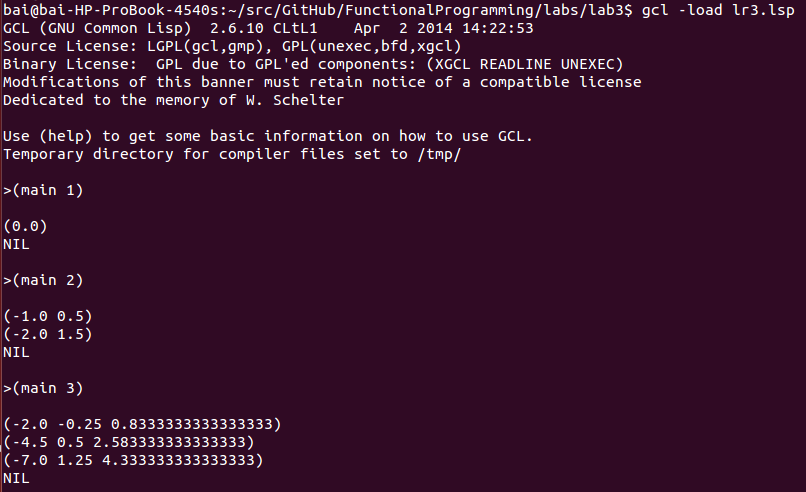
\includegraphics[scale=0.5]{lr3Screen}

%\subsection{Результаты работы}
%\lstinputlisting{./log2.lsp}

\section{Дневник отладки}
\begin{tabular}{|c|p{5cm}|p{5cm}|p{3cm}|}
\hline
Дата & Событие & Действие по исправлению & Примечание \\
\hline
11.05.2016 & BugFix & Изменил ограничение в одном из циклов при перемножении матриц (самый вложенный), не смотря на то, что это никак не влияло на результат, т.к. матрицы квадратные. & Исправления были добавлены для унификации функции произведения матриц. \\
11.05.2016 & Refactoring & Заменил {\color{red}\tt{(- 1.0)}} на {\color{green}\tt{-1.0}} &  \\
11.05.2016 & Refactoring & Вынес в глобальную область ф-ию {\color{red}\tt{GetListFromMatrix}} & \\
11.05.2016 & Refactoring & Убрал вшитую в код размерность матрицы, теперь можно подавать на вход программе \tt{(main n)} &  \\
\hline 
\end{tabular}

\section{Замечания, выводы}
Мною была также написана ф-ия для <<красивого>> вывода матрицы {\color{red} PrintMatrix} (на мой взгляд). В результатах работы программы матрица $\mathbb{A}_{3\times3}$. 
\[
\mathbb{A}=\begin{bmatrix}
			1 & 2 & 3\\
			4 & 5 & 6\\
			7 & 8 & 9
			\end{bmatrix}
,
\mathbb{B}=\begin{bmatrix}
			0 & \frac{1}{2} & \frac{1}{3}\\
			-\frac{1}{2} & 0 & \frac{1}{4}\\
			-\frac{1}{3} & -\frac{1}{4} & 0
			\end{bmatrix}
\]
Для демонстрации корректности результата, я прикрепляю скриншот с сайта, на котором реализован алгоритм произведения матриц:\\
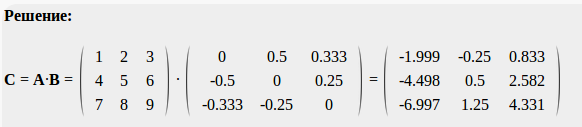
\includegraphics[scale=0.5]{lr3Prove}

\end{document}
